\documentclass{amsart}
%\documentclass[a4paper,10pt]{scrartcl}

\usepackage[utf8x]{inputenc}
\usepackage[british]{babel}
%\usepackage[a4paper, inner=0.5cm, outer=0.5cm, top=1cm,
%bottom=1.5cm, bindingoffset=1cm]{geometry}
\usepackage{amsmath}
\usepackage{amssymb, latexsym}
\usepackage{longtable}
\usepackage[table]{xcolor}
\usepackage{textcomp} 
\usepackage{stmaryrd}
\usepackage{graphicx}
\usepackage{enumitem}
\usepackage{yfonts}
\usepackage{algpseudocode}
\usepackage{algorithm}
\usepackage{hyperref}
\usepackage{MnSymbol}

\setlist[enumerate]{label*=\arabic*.}
\newtheorem{theorem}{Theorem}[section]
\newtheorem{example}{Example}[section]
\newtheorem{definition}{Definition}[section]
\newtheorem{proposition}{Proposition}[section]
\newtheorem{notation}{Notation}[section]

\renewcommand{\algorithmicrequire}{\textbf{Input:}}
\renewcommand{\algorithmicensure}{\textbf{Output:}}

\title{Understanding OWL Existential Property Restrictions}
\author{Henriette Harmse}
\date{\today}

\pdfinfo{%
  /Title    (Understanding OWL Existential Property Restrictions)
  /Author   (Henriette Harmse)
  /Creator  ()
  /Producer ()
  /Subject  (DL)
  /Keywords ()
}

\begin{document}
  \maketitle
  
  For many starting out with OWL ontologies understanding the exact meaning of property restrictions can be challenging. In this post I will use visual representations to explain the meaning of existential property restrictions. For the purpose of this post, we start out with a simple ontology for modelling the relation between a person and their pets.  You can model this in the free \href{https://protege.stanford.edu/products.php}{Prot\'{e}g\'{e}} ontology editor.
  
\begin{small}
\begin{verbatim} 
ObjectProperty: owns
        
Class: Cat
  SubClassOf: Pet
    
Class: Dog
  SubClassOf: Pet
    
Class: Person
  DisjointWith: Pet
        
Class: Pet
  DisjointUnionOf: Cat, Dog
  DisjointWith: Person    
\end{verbatim}
\end{small}  

I have specified this ontology using the \href{http://www.w3.org/TR/owl2-manchester-syntax/}{OWL 2 Manchester syntax}. Other syntax can be used as well, notably the functional-style syntax, which is used to define the \href{https://www.w3.org/TR/owl2-direct-semantics/}{direct semantics of OWL 2}. In this post I use the Manchester syntax because it tends to be more intuitive to non-logicians, but it has some weaknesses which I will point out when we get to it. Also for clarity and compactness I have omitted the prefixes.

This ontology states that in our domain we have persons (\texttt{Class: Person}) and pets (\texttt{Class: Pet}). Persons cannot be pets, and pets cannot be persons (\texttt{Class: Pet DisjointWith: Person}). Cats (\texttt{Class: Cat SubClassOf: Pet}) and dogs (\texttt{Class: Dog SubClassOf: Pet}) are pets. We further assume that cats and dogs are the only pets in our domain, and a cat is not a dog and vice versa (\texttt{Class: Pet  DisjointUnionOf: Cat, Dog}). I have also defined an \texttt{owns} object property, which will be the basis of our discussions on existential property restrictions. You can run the reasoner to confirm for yourself that this ontology is indeed consistent, that is, it contains no logical contradictions.
  
  In this post I will explain through visual representations what is the meaning of
  \begin{enumerate}
   \item \texttt{owns some owl:Thing},
   \item \texttt{Class: AnimalLover SubClassOf: owns some owl:Thing},
   \item \texttt{owns some owl:Thing SubClassOf: AnimalLover}, and
   \item \texttt{Class: AnimalLover EquivalentTo: owns some Pet}.
   \end{enumerate}

  
  \section{owns some owl:Thing}
  One of the first things one has to realize working with OWL ontologies is that OWL describes sets (in OWL called classes) and relations (in OWL called properties) between sets for some domain of interest. A domain of interest consists of elements (in OWL called individuals) that can belong to classes and/or form part of properties. The domain of interest represents the largest set of individuals that we are interested in, which in OWL is represented by \texttt{owl:Thing}. The smallest set we are interested in is the empty set, which in OWL is represented by \texttt{owl:Nothing}.
  
    \begin{figure}
    %trim option's parameter order: left bottom right top
      \centering 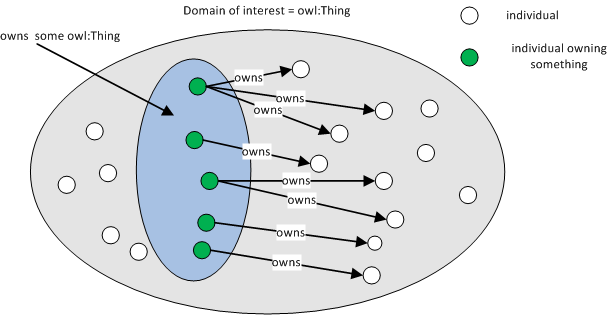
\includegraphics[trim = 0mm 0mm 0mm 0mm, clip, scale=1]{./ownsSomeThing.png}
      \caption{\texttt{owns some owl:Thing}}\label{fig_ownsSomeThing}
    \end{figure}  
    
  In Figure~\ref{fig_ownsSomeThing} I have illustrated an example domain consisting of some individuals (the small circles) and some \texttt{owns} properties (the arrows) that exist between individuals. At this stage I have not indicated the \texttt{Person} or \texttt{Pet} classes as yet. The meaning of \texttt{owns some owl:Thing} is that it represents the set of those individuals that we know owns something. In our example it consists of the individuals represented by the green circles (i.e. 5 individuals). Note that due to the \texttt{open world assumption}, we cannot assume that individuals that do not form part of the \texttt{owns} property, necessarily do not own anything. Rather, OWL reasoners assume that it is not know whether these individuals own something or do not own something. Because \texttt{owns some owl:Thing} represents a set OWL reasoners and ontology editors some times refer to an expression like \texttt{owns some owl:Thing} as an \texttt{anonymous class}. I.e. it is a class just like \texttt{Person}, but unlike \texttt{Person} it does not have name.
  
  
  To refer specifically to owners of pets we have to define our existential property restriction as \texttt{owns some Pet}. This is illustrated in Figure~\ref{fig_ownsSomePet}. As you can see \texttt{owns some Pet} is a subset (subclass) of \texttt{owns some owl:Thing}. 
  
    \begin{figure}
    %trim option's parameter order: left bottom right top
      \centering 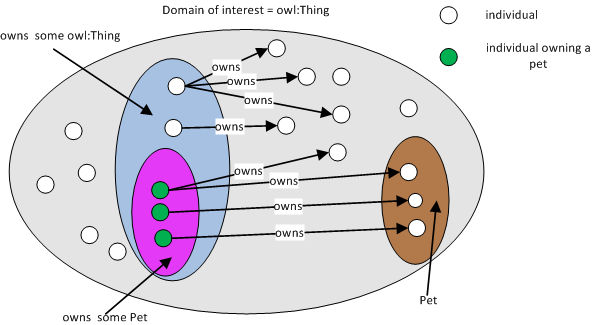
\includegraphics[trim = 0mm 0mm 0mm 0mm, clip, scale=1]{./ownsSomePet.png}
      \caption{\texttt{owns some Pet}}\label{fig_ownsSomePet}
    \end{figure}    
  
  \section{Class: AnimalLover SubClassOf: owns some Pet}
  Assume now we want to model a person that loves animals as someone who has at least 1 pet. We can model this as follows:
\begin{small}
\begin{verbatim} 
Class: AnimalLover
  SubClassOf: 
    Person,
    owns some Pet
\end{verbatim}
\end{small}  
To test our ontology we create an individual without a pet.
\begin{small}
\begin{verbatim} 
Individual: anAnimalLoverWithoutAPet
  Types: AnimalLover
\end{verbatim}
\end{small} 
Since our \texttt{anAnimalLoverWithoutAPet} individual is defined as belonging to the \texttt{AnimalLover} class and we have not stated that it owns a pet, we may expect that the reasoner will find our ontology inconsistent. However, this is not the case. The reason for this is again due to the open world assumption: there is nothing in our ontology that states that the \texttt{anAnimalLoverWithoutAPet} individual has no pets. To make explicit that \texttt{anAnimalLoverWithoutAPet} owns no pets, we change our definition of \texttt{anAnimalLoverWithoutAPet} as follows
\begin{small}
\begin{verbatim} 
Individual: anAnimalLoverWithoutAPet
  Types: 
    AnimalLover, 
    owns max 0 Pet
\end{verbatim}
\end{small} 
which states that \texttt{anAnimalLoverWithoutAPet} has a maximum of zero pets. If we now run the reasoner it will give an inconsistency. When your ontology gives an inconsistency (even when you expect it), it is good idea to check whether it gives an inconsistency for the correct reasons. This will help you to confirm whether you designed your ontology correctly for your desired outcomes. In this case the explanation for the inconsistency is given in Figure~\ref{fig_ExplanationAnimalLoverWithoutAPet}:
    \begin{figure}
    %trim option's parameter order: left bottom right top
      \centering 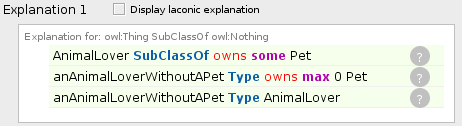
\includegraphics[trim = 0mm 0mm 0mm 0mm, clip, scale=0.6]{./ExplanationAnimalLoverWithoutAPet.png}
      \caption{Explanation for an animal lover not owning a pet}\label{fig_ExplanationAnimalLoverWithoutAPet}
    \end{figure} 
It states that the inconsistency is due to the following reasons: (1) \texttt{anAnimalLoverWithoutAPet} is an animal lover (\texttt{anAnimalLoverWithoutAPet Types AnimalLover}), (2) who does not own a pet \texttt{ anAnimalLoverWithoutAPet Types owns max 0 owl:Thing}, (3) but the expectation is that an animal lover should own a pet (\texttt{AnimalLover SubClassOf owns some Pet}).

Explanations are minimal. That means that if you remove any 1 of the reasons given in an explanation, it is no longer an explanation for the inconsistency (or an entailment). Hence, 
\begin{small}
\begin{verbatim} 
anAnimalLoverWithoutAPet Type AnimalLover
AnimalLover owns some Pet
\end{verbatim}
\end{small} 
is \textbf{not} an explanation for the inconsistency. This gives us a hint on how to remove an inconsistency from an ontology. If we can change our ontology such that any of the reasons given in an explanation for an inconsistency no longer holds, our ontology will be consistent. In this case we can (again) remove the \texttt{owns max 0 Pet} type from \texttt{anAnimalLoverWithoutAPet}.



An incorrect assumption we may make based on the design of our ontology is that when ever an individual has a pet, the reasoner will infer that the individual is an \texttt{AnimalLover}. However, as I said, this assumption is incorrect. Thus, changing our ontology as follows

\begin{small}
\begin{verbatim} 
Individual: aCat
  Types: Cat

Individual: aPetOwner
  Facts: 
    owns aCat
\end{verbatim}
\end{small} 
will not result in inferring that \texttt{aPetOwner} is an \texttt{AnimalLover}.

To understand this see Figure~\ref{fig_SubClassOfOwnsSomePet}. Because we have defined \texttt{AnimalLover} as a subclass of \texttt{owns some Pet} it means the following possibilities exist:
\begin{enumerate}
 \item There may be persons who have pets who do not love animals.
 \item There may be individuals that have pets who are not persons.
\end{enumerate}
Hence, from our current ontology, the reasoner can infer nothing more.

    \begin{figure}
    %trim option's parameter order: left bottom right top
      \centering 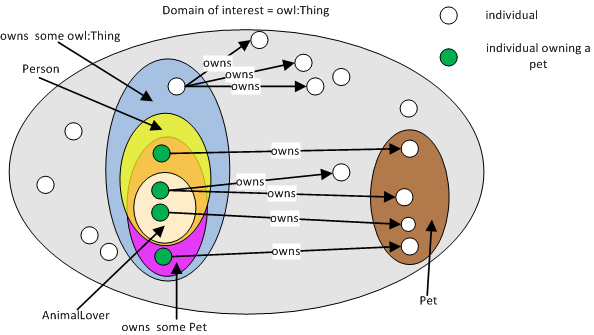
\includegraphics[trim = 0mm 0mm 0mm 0mm, clip, scale=0.6]{./SubClassOfOwnsSomePet.png}
      \caption{\texttt{AnimalLover SubClassOf: owns some Pet}}\label{fig_SubClassOfOwnsSomePet}
    \end{figure} 
  
  \section{owns some Pet SubClassOf: AnimalLover}
  Now in this section, instead of defining \texttt{AnimalLover} as a subclass of \texttt{owns some Pet}, let us use a general class axiom and define \texttt{owns some Pet SubClassOf: AnimalLover} with \texttt{AnimalLover} defined as follows:
\begin{small}
\begin{verbatim} 
Class: AnimalLover
  SubClassOf: Person
\end{verbatim}
\end{small}   
Note that if you now save your ontology in Manchester syntax, you will loose the \texttt{owns some Pet SubClassOf: AnimalLover} general class axiom. Rather save it in say RDF/XML or OWL/XML syntax. We also add the following individuals:
\begin{small}
\begin{verbatim} 
Individual: aCat

Individual: aPetOwner
  Facts: 
    owns aCat
\end{verbatim}
\end{small}  
Ensure that you have specified no type information for \texttt{aCat} and \texttt{aPetOwner}. If you run the reasoner it will not infer that \texttt{aCat} is of type \texttt{Cat}. This is because \texttt{aCat} is not of type \texttt{Cat}. If you state that \texttt{aCat} is of type \texttt{Cat}, it will infer that \texttt{aPetOwner} is an \texttt{AnimalLover}.

One reason why this design may not be ideal is that if we again consider the case where an individual \texttt{anAnimalLoverWithoutAPet} of type \texttt{AnimalLover} does not have a pet (as defined in the previous section), it will not give an inconsistency. 
To understand the reason why the reasoner cannot make this inference, see Figure~\ref{fig_OwnsSomePetSubclassAnimalLover}.
    \begin{figure}
    %trim option's parameter order: left bottom right top
      \centering 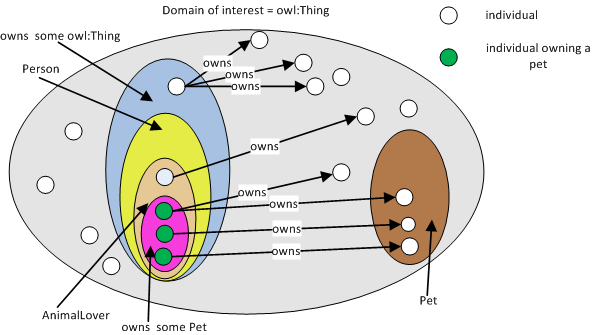
\includegraphics[trim = 0mm 0mm 0mm 0mm, clip, scale=0.6]{./OwnsSomePetSubclassAnimalLover.png}
      \caption{\texttt{owns some Pet SubClassOf: AnimalLover}}\label{fig_OwnsSomePetSubclassAnimalLover}
    \end{figure} 
Because we defined \texttt{owns some Pet SubClassOf: AnimalLover} the possibility exists that there are \texttt{AnimalLover}s who do not own any pets.

  \section{Class: AnimalLover EquivalentTo: owns some Pet}
 From the previous 2 sections we have noted that defining \texttt{AnimalLover} as \texttt{AnimalLover SubClassOf: owns some Pet} and 
 \texttt{own some Pet SubClassOf: AnimalLover} each have benefits and downsides. If only we could define \texttt{AnimalLover} in terms of both. This can be achieved by defining \texttt{AnimalLover} as follows:
\begin{small}
\begin{verbatim} 
Class: AnimalLover
  EquivalentTo: owns some Pet
\end{verbatim}
\end{small}  
With this definition in place, an individual who owns a pet will be inferred to be of type \texttt{AnimalLover}. If an individual is of type \texttt{AnimalLover}, but it is known to have no pets, it will cause an inconsistency. The reason way this definition is not suffering of the problems we encountered with our previous approaches is because the \texttt{AnimalLover} class is now equivalent to the  \texttt{owns some Pet} class.

Does this mean it is better to define classes in terms of equivalence rather than subclasses? No. In this instance it turned out to be the case only because we made the assumption that \texttt{AnimalLover}s are equivalent to someone owning a pet. Clearly in reality there may be people owning pets but who do not like pets. Hence, given other assumptions a different ontology may have been a better choice.

  \section{Conclusion}
The purpose of this post is to explain the meaning of existential property restrictions. For this reason I did not consider using domain and range restrictions to enable inferring that someone who owns a pet is necessarily an \texttt{AnimalLover}. This can easily be achieved by stating 
\begin{small}
\begin{verbatim} 
ObjectProperty: owns
  Domain: AnimalLover
  Range: Pet
\end{verbatim}
\end{small}  
However, domain and range restrictions are really just syntactical sugar that can be expressed in terms of existential property restrictions (or universal property restrictions).  
 
The example ontologies of this post can be found in \href{https://github.com/henrietteharmse/henrietteharmse/tree/master/blog/tutorial/ontologies/docs/Understanding\%20OWL\%20Existential\%20Property\%20Restrictions}{github}.

  \bibliographystyle{amsplain}
  \bibliography{../../../BibliographicDetails_v.0.1}
 
\end{document}
